\mychapter{함수}{}
\section{대응과 함수}  
\subsection{대응의 정의}
두 집합 $X$, $Y$에 대하여 집합 $X$의 원소에 집합 $Y$의 원소를 짝 지어 주는 것을 `$X$에서 $Y$로의 \term{대응}{}'이라고 합니다. 이때 집합 $X$의 원소 $x$에 집합 $Y$의 원소 $y$가 짝 지어지면 `$x$에 $y$가 \term{대응한다}{}'고 하며, 이것을 기호로 $x \longrightarrow y$와 같이 나타냅니다.

\subsection{함수의 정의}
두 집합 $X$, $Y$에 대하여 집합 $X$의 각 원소에 집합 $Y$의 원소가 오직 하나씩만 대응할 때, 이 대응을 `$X$에서 $Y$로의 \term{함수}{}'라고 합니다. 이를 기호로 나타내면 다음과 같습니다.\mn{함수의 이름은 관습적으로 $f$, $g$, $h$와 같이 짓습니다. 함수의 영문 이름이 function이기 때문입니다.}{}
\begin{align*} f : X \longrightarrow Y\end{align*}

\subsection{함수의 정의에 대한 추가설명}
함수의 정의는 문장의 길이가 짧음에도 불구하고 굉장히 깐깐한 제약조건을 담고 있습니다. 문장 성분별로 분석하여 대응이 함수가 되기 위한 제약조건을 알아보고, 제약조건으로 착각하기 쉽지만 제약조건이 아닌 것을 알아봅시다.

\begin{figure}[h]\centering \subfloat[][]{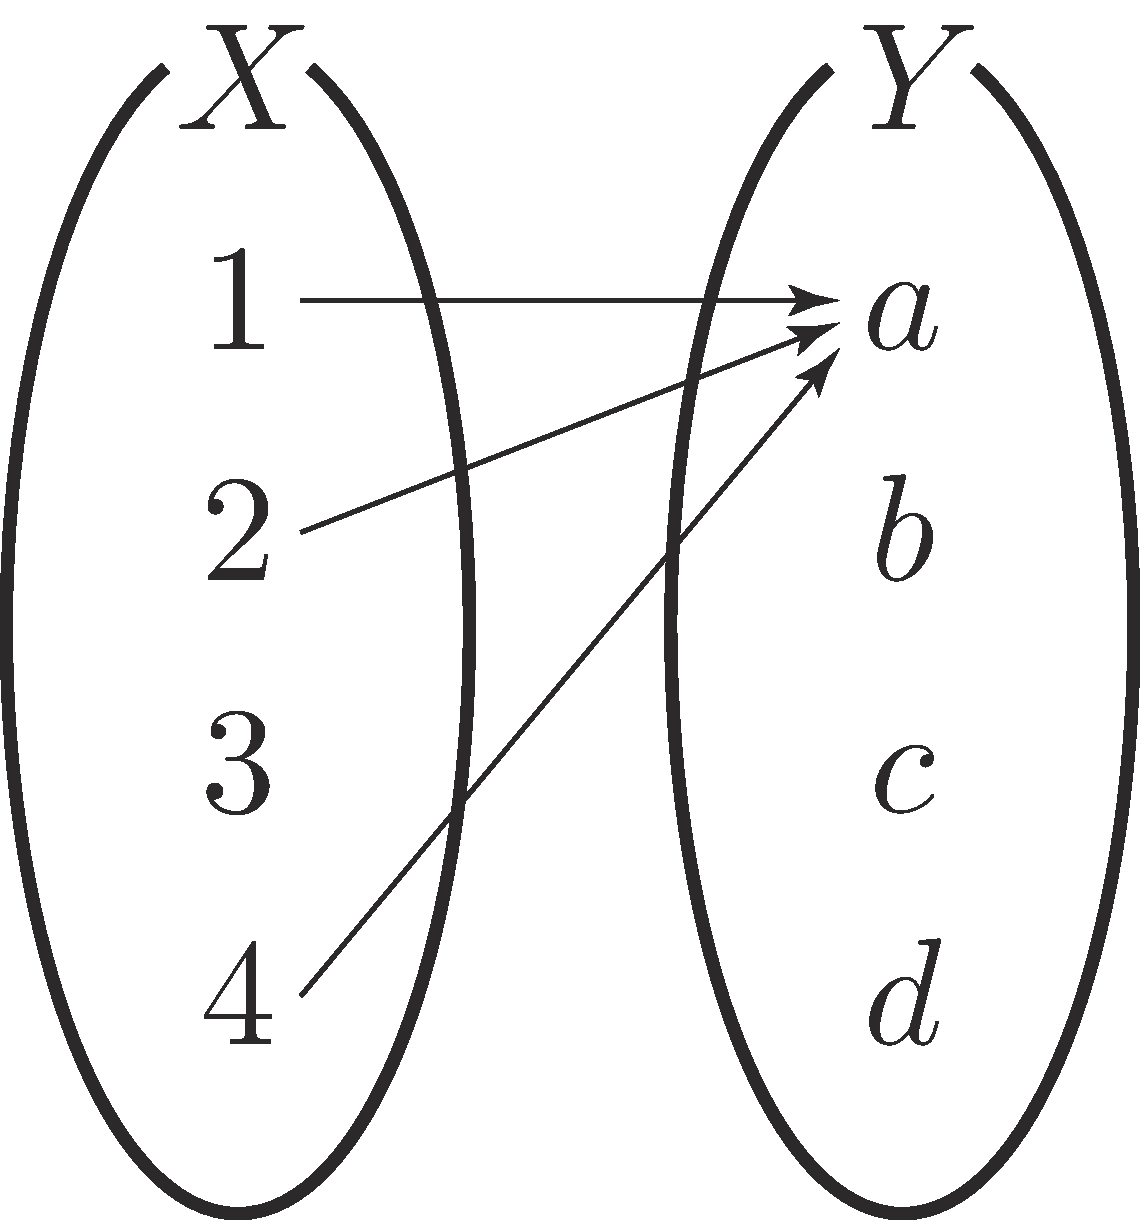
\includegraphics[scale=\pgfkeysvalueof{picsize}]{DBs/pic/zerg_01_1.pdf}}\
\qquad
\centering \subfloat[(2)][]{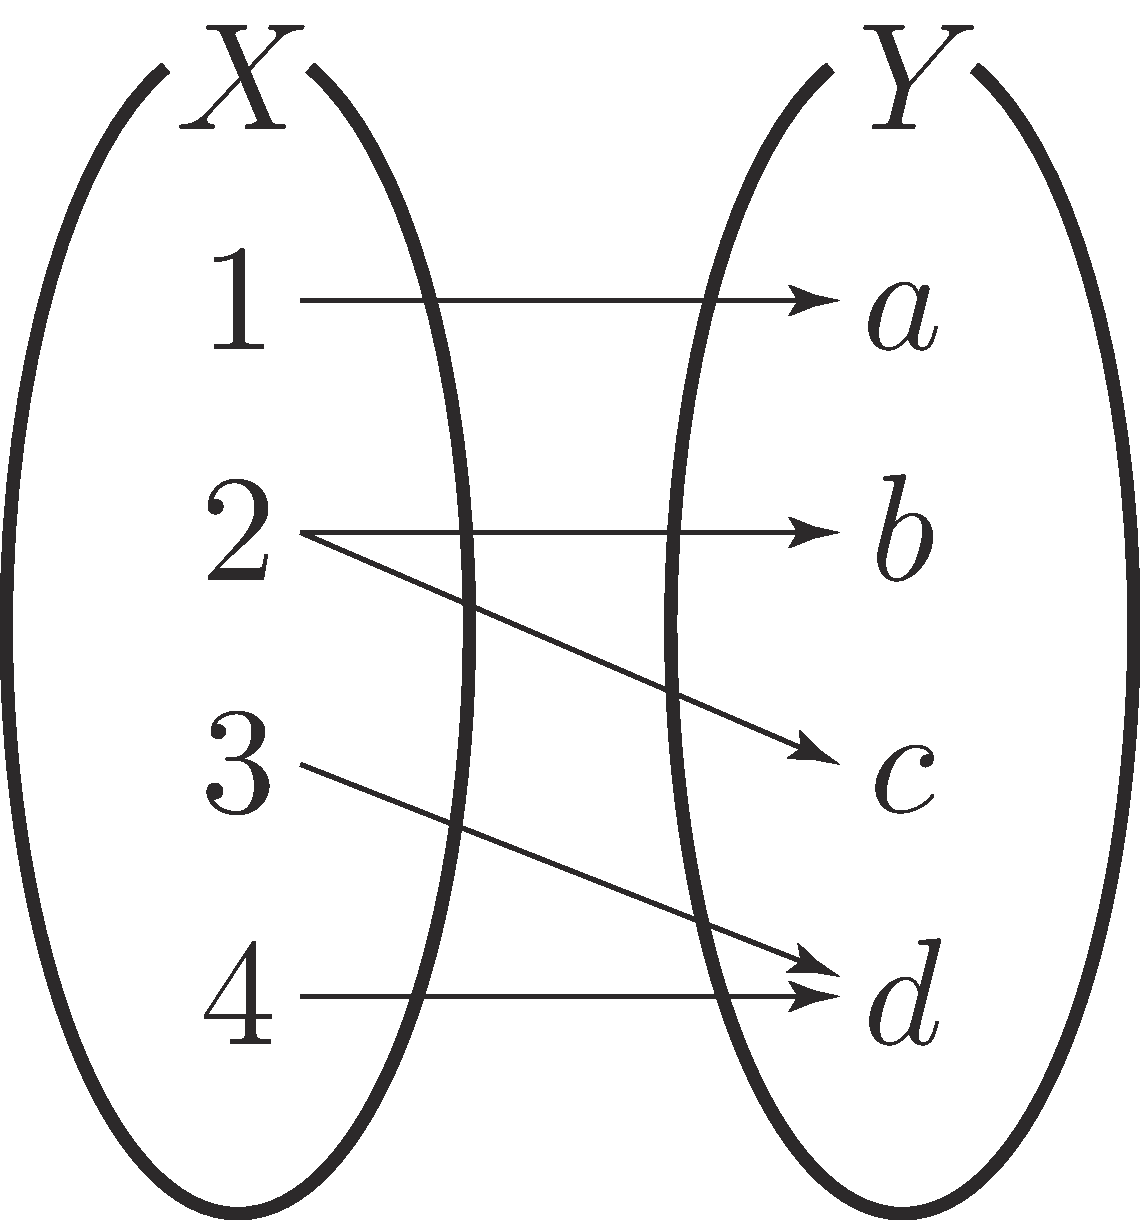
\includegraphics[scale=\pgfkeysvalueof{picsize}]{DBs/pic/zerg_01_2.pdf}}\
\qquad
\centering \subfloat[][]{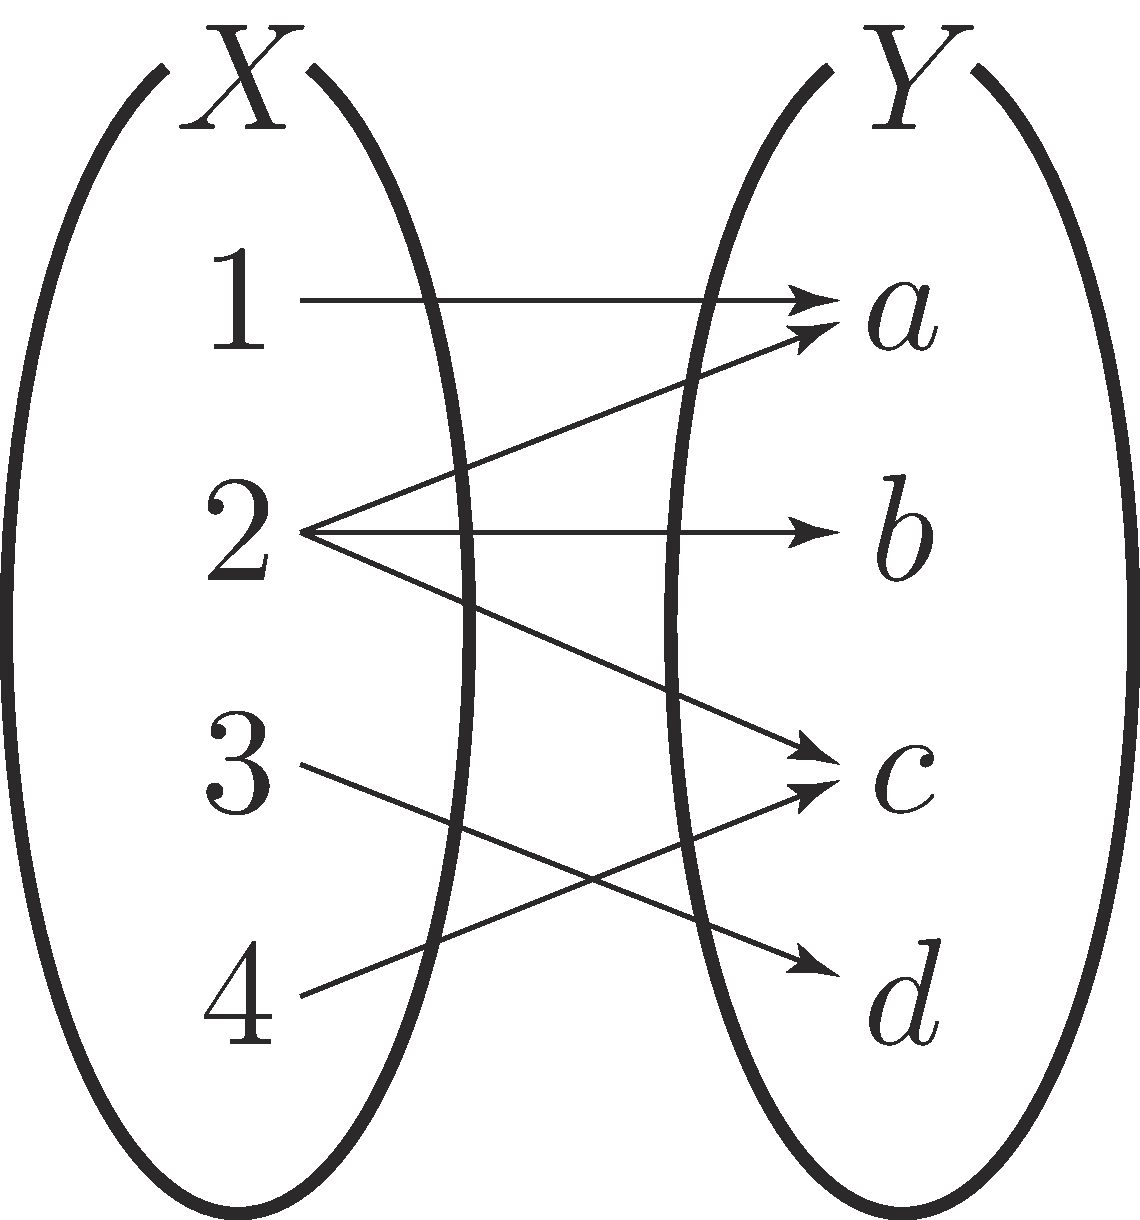
\includegraphics[scale=\pgfkeysvalueof{picsize}]{DBs/pic/zerg_01_3.pdf}}\
\qquad
\centering \subfloat[][]{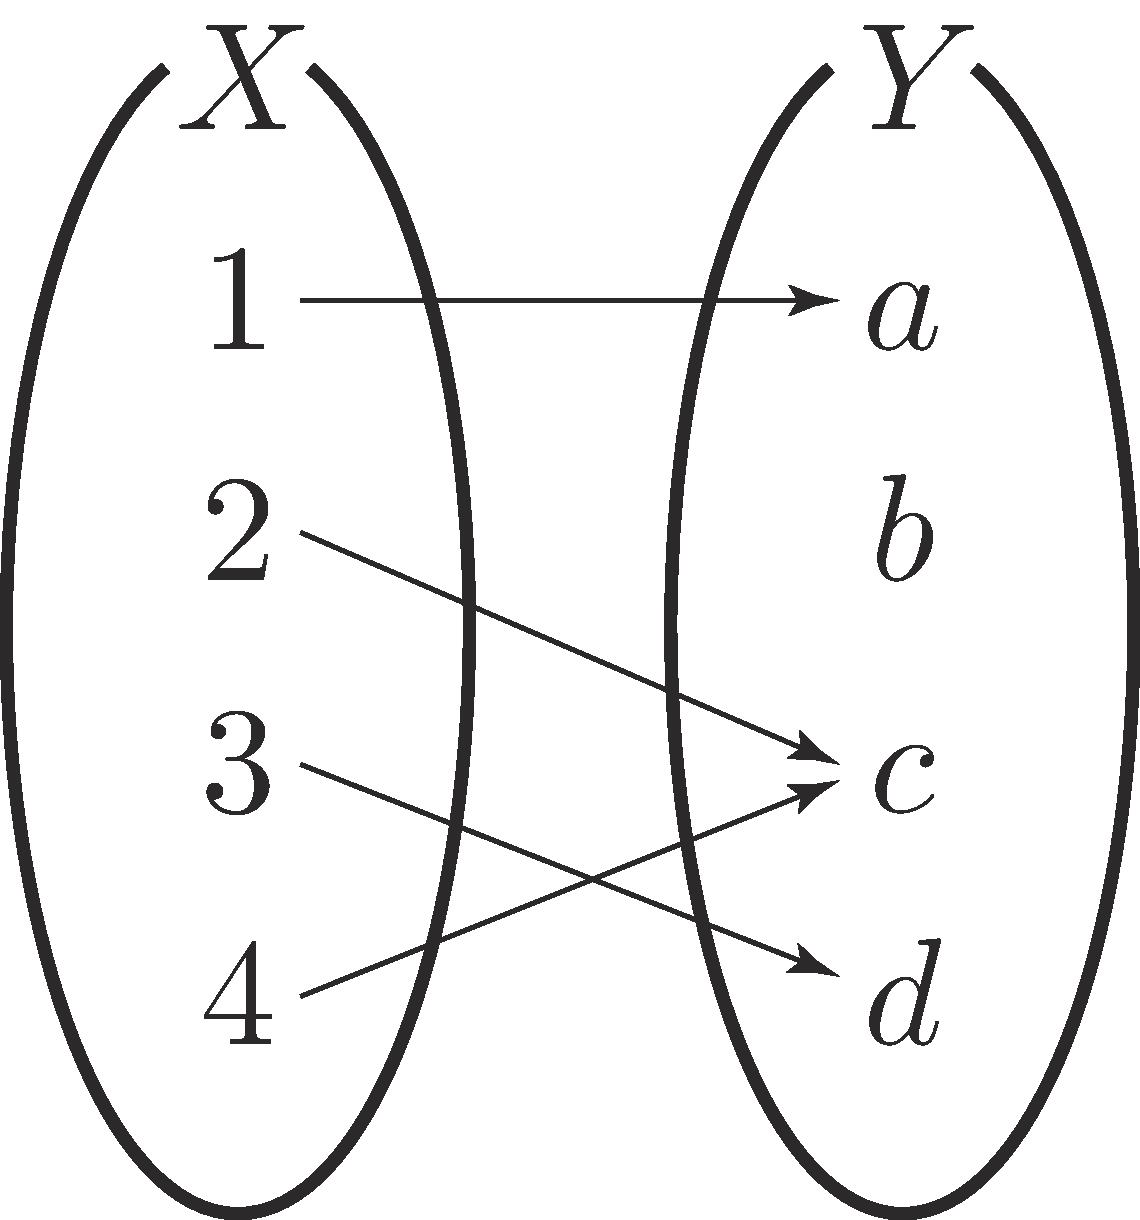
\includegraphics[scale=\pgfkeysvalueof{picsize}]{DBs/pic/zerg_01_4.pdf}}\
\end{figure}
\subsubsection{제약조건 (1) : 집합 $X$의 `각' 원소}
대응은 $X$의 원소 중 단 하나만 $Y$의 원소와 대응되더라도 관계없었습니다. 그러나 함수는 $X$의 각 원소가 하나도 빠짐없이 $Y$의 원소에 대응되어야 합니다. 

그림 (a)의 대응은 함수가 아닙니다. $X$의 원소인 $3$에 대응되는 $Y$의 원소가 없기 때문입니다.\mn{만약 집합 $Z=\left\{1,\: 2,\: 4\right\} $을 생각한다면 그림 (a)와 같은 상황에서 함수 $g:Z \longrightarrow Y$를 생각할 수는 있습니다.}{}  이와 달리 그림 (d)의 대응은 함수입니다.
\clearpage
\subsubsection{제약조건 (2) : 집합 $Y$의 원소가 `오직 하나씩만'}
대응은 $X$의 원소 하나에 $Y$의 원소 여러개가 대응되더라도 상관없었습니다. 함수는 $X$의 원소 하나에 대응되는 $Y$의 원소가 오직 하나여야(유일해야) 합니다. 

그림 (b), (c)의 대응은 함수가 아닙니다. `$X$의 원소인 $2$에 대응하는 $Y$의 원소'의 개수가 각각 $2$, $3$이기 때문입니다. 이와 달리 그림 (d)의 대응은 함수입니다.

\subsubsection{제약조건이 아닌 것 : $Y$의 모든 원소가 대응될 필요는 없다}
대응에서 $Y$의 모든 원소가 빠짐없이 대응될 필요는 없었듯이, 함수에서도 마찬가지입니다. 대응이 함수가 되기 위한 제약조건은 $X$의 원소, 그리고 $X$에 대응되는 $Y$의 원소에만 국한될 뿐임을 주의합시다.

\section{함수 관련 용어의 정의}
\subsection{정의역, 공역, 치역, 함숫값}
집합 $X$, $Y$와 함수 $f : X \longrightarrow Y$에 대하여 $X$를 함수 $f$의 \term{정의역}{}, $Y$를 함수 $f$의 \term{공역}{}이라 합니다. 또한 함수 $f$에 의하여 정의역의 원소 $x$에 공역의 원소 $y$가 대응할 때, 이를 등식으로 $y=f\left( x \right) $와 같이 나타내고, $f(x)$를 $x$에서의 \term{함숫값}{}이라고 합니다. 이때 함숫값 전체의 집합인 $\conset{f\left( x \right) }{$x\in X$}$를 함수 $f$의 \term{치역}{}이라고 합니다.

\subsection{`제약조건'과 정의역, 함숫값}
제약조건 (1)에 따르면, 정의역에 포함된 임의의 원소 $x$에 대하여 함숫값 $f(x)$가 항상 존재합니다. 제약조건 (2)에 따르면, 정의역에 포함된 임의의 원소 $x$에 대하여 $f(x)$의 값은 유일합니다.\mn{이 문장에서 말하는 것은 `$x$의 값에 관계 없이 $f(x)$의 값이 같다'는 것이 아니라, $f(3)=3$인 동시에 $f(3)=5$일 수 없다는 것입니다. `$x$의 값에 관계 없이 $f(x)$의 값이 같은 함수'에 대해서는 곧 뒤에서 배웁니다.}{} 


\subsection{`제약조건이 아닌 것'과 치역, 공역}
어떤 함수의 공역을 $Y$, 치역을 $F$라 할 때, `제약조건이 아닌 것'에 따르면, 치역과 공역이 항상 일치하는 것은 아닙니다. 한편, 치역은 $Y$의 원소 중에서 함숫값 $f(x)$가 될 수 있는 원소들로 이루어진 집합이므로, 치역은 공역의 부분집합입니다. 따라서 $F$가 $Y$의 진부분집합이면 공역과 치역이 일치하지 않습니다.

\subsection{정의역과 공역의 범위}
함수 $y=f\left( x \right) $의 정의역과 공역이 주어진 경우에는 정의역과 공역의 범위를 주어진 대로 취합니다. 함수 $y=f\left( x \right) $의 정의역과 공역이 주어지지 않는 경우에는 특별한 이유가 없는 한 $f(x)$가 정의되는 실수 $x$의 값 전체의 집합을 정의역으로, 실수 전체의 집합을 공역으로 생각합니다.\mn{특별한 이유의 대표적인 예시는 `일대일함수를 일대일대응이 되도록 공역을 치역에 맞추어 축소시키기'가 있습니다.}{}
\clearpage
\section{함수의 서로 같음}
두 함수 $f$, $g$가 다음을 만족시킬 때, `두 함수 $f$, $g$는 \term{서로 같다}{}'고 하고, $f=g$와 같이 나타냅니다.
\begin{justbox}
    \begin{enumerate}[label={\onum*}]
            \item 정의역과 공역이 각각 서로 같다.
            \item 정의역의 모든 원소 $x$에 대하여 $f(x)=g(x)$이다.
        \end{enumerate}
\end{justbox}
예를 들어 $f\left( x \right) =\dfrac{x^2-1}{x-1}$과 $g\left( x \right) =x+1$는 $x\ne1$인 모든 실수 $x$에 대하여 $f\left( x \right)=g\left( x \right)$가 성립하므로 두 함수 $f$, $g$가 서로 같다고 착각하기 쉽습니다. 그러나 정의역이 같을 수 없으므로\mn[-3\blskip]{단, $f$와 $g$의 정의역에서 $x = 1$을 제외해주면 정의역을 같게 해줄 수 있습니다.}{} 두 함수 $f$, $g$는 서로 같지 않습니다.

\section{함수의 그래프} 
함수 $f:X \longrightarrow Y$에서 정의역 $X$의 원소 $x$와 이에 대응하는 함숫값 $f(x)$의 순서쌍 $\xy{x}{f(x)}$ 전체의 집합 $G=\conset{\xy{x}{f\left( x \right) }}{$x \in X$}$를 함수 $f$의 \term{그래프}{}라고 합니다.\mn[-2\blskip]{그래프를 그림 그 자체라고 생각하는 경우가 많지만, 정의에 따르면 그래프는 집합이지 그림이 아닙니다. 그림은 그 집합을 좌표평면에 나타내었을 때 드러나는 형상일 뿐입니다.}{}  정의역과 치역이 각각 $\mathbb{R}$의 부분집합인 함수 $y=f(x)$의 그래프는 순서쌍 $\xy{x}{f\left( x \right) }$를 좌표평면에 점으로 나타내어 그릴 수 있습니다.
\clearpage
\section{여러 가지 함수}
\subsection{일대일함수와 일대일대응}
다음 조건을 만족시키는 함수 $f: X \longrightarrow Y$를 \term{일대일함수}{}라 합니다.
\begin{justbox}
    정의역 $X$의 임의의 두 원소 $x_1$, $x_2$에 대하여 $x_1 \ne x_2$이면 $f\left( x_1 \right) \ne f\left( x_2 \right) $이다.
\end{justbox}
다음 조건을 만족시키는 함수 $f: X \longrightarrow Y$를 \term{일대일대응}{}이라 합니다.\mn{교과서에서는 `일대일 대응'으로 띄어쓰고 있지만, 그 띄어쓰기의 기준이 일관되지 않습니다. 따라서 불필요한 혼동을 피하기 위하여 붙여쓰도록 하겠습니다.}{}
\begin{justbox}
    \begin{enumerate}[label=\onum*]
        \item $f$가 일대일함수이다.
        \item $f$의 공역과 치역이 서로 같다. 
    \end{enumerate}
\end{justbox}

\begin{center} 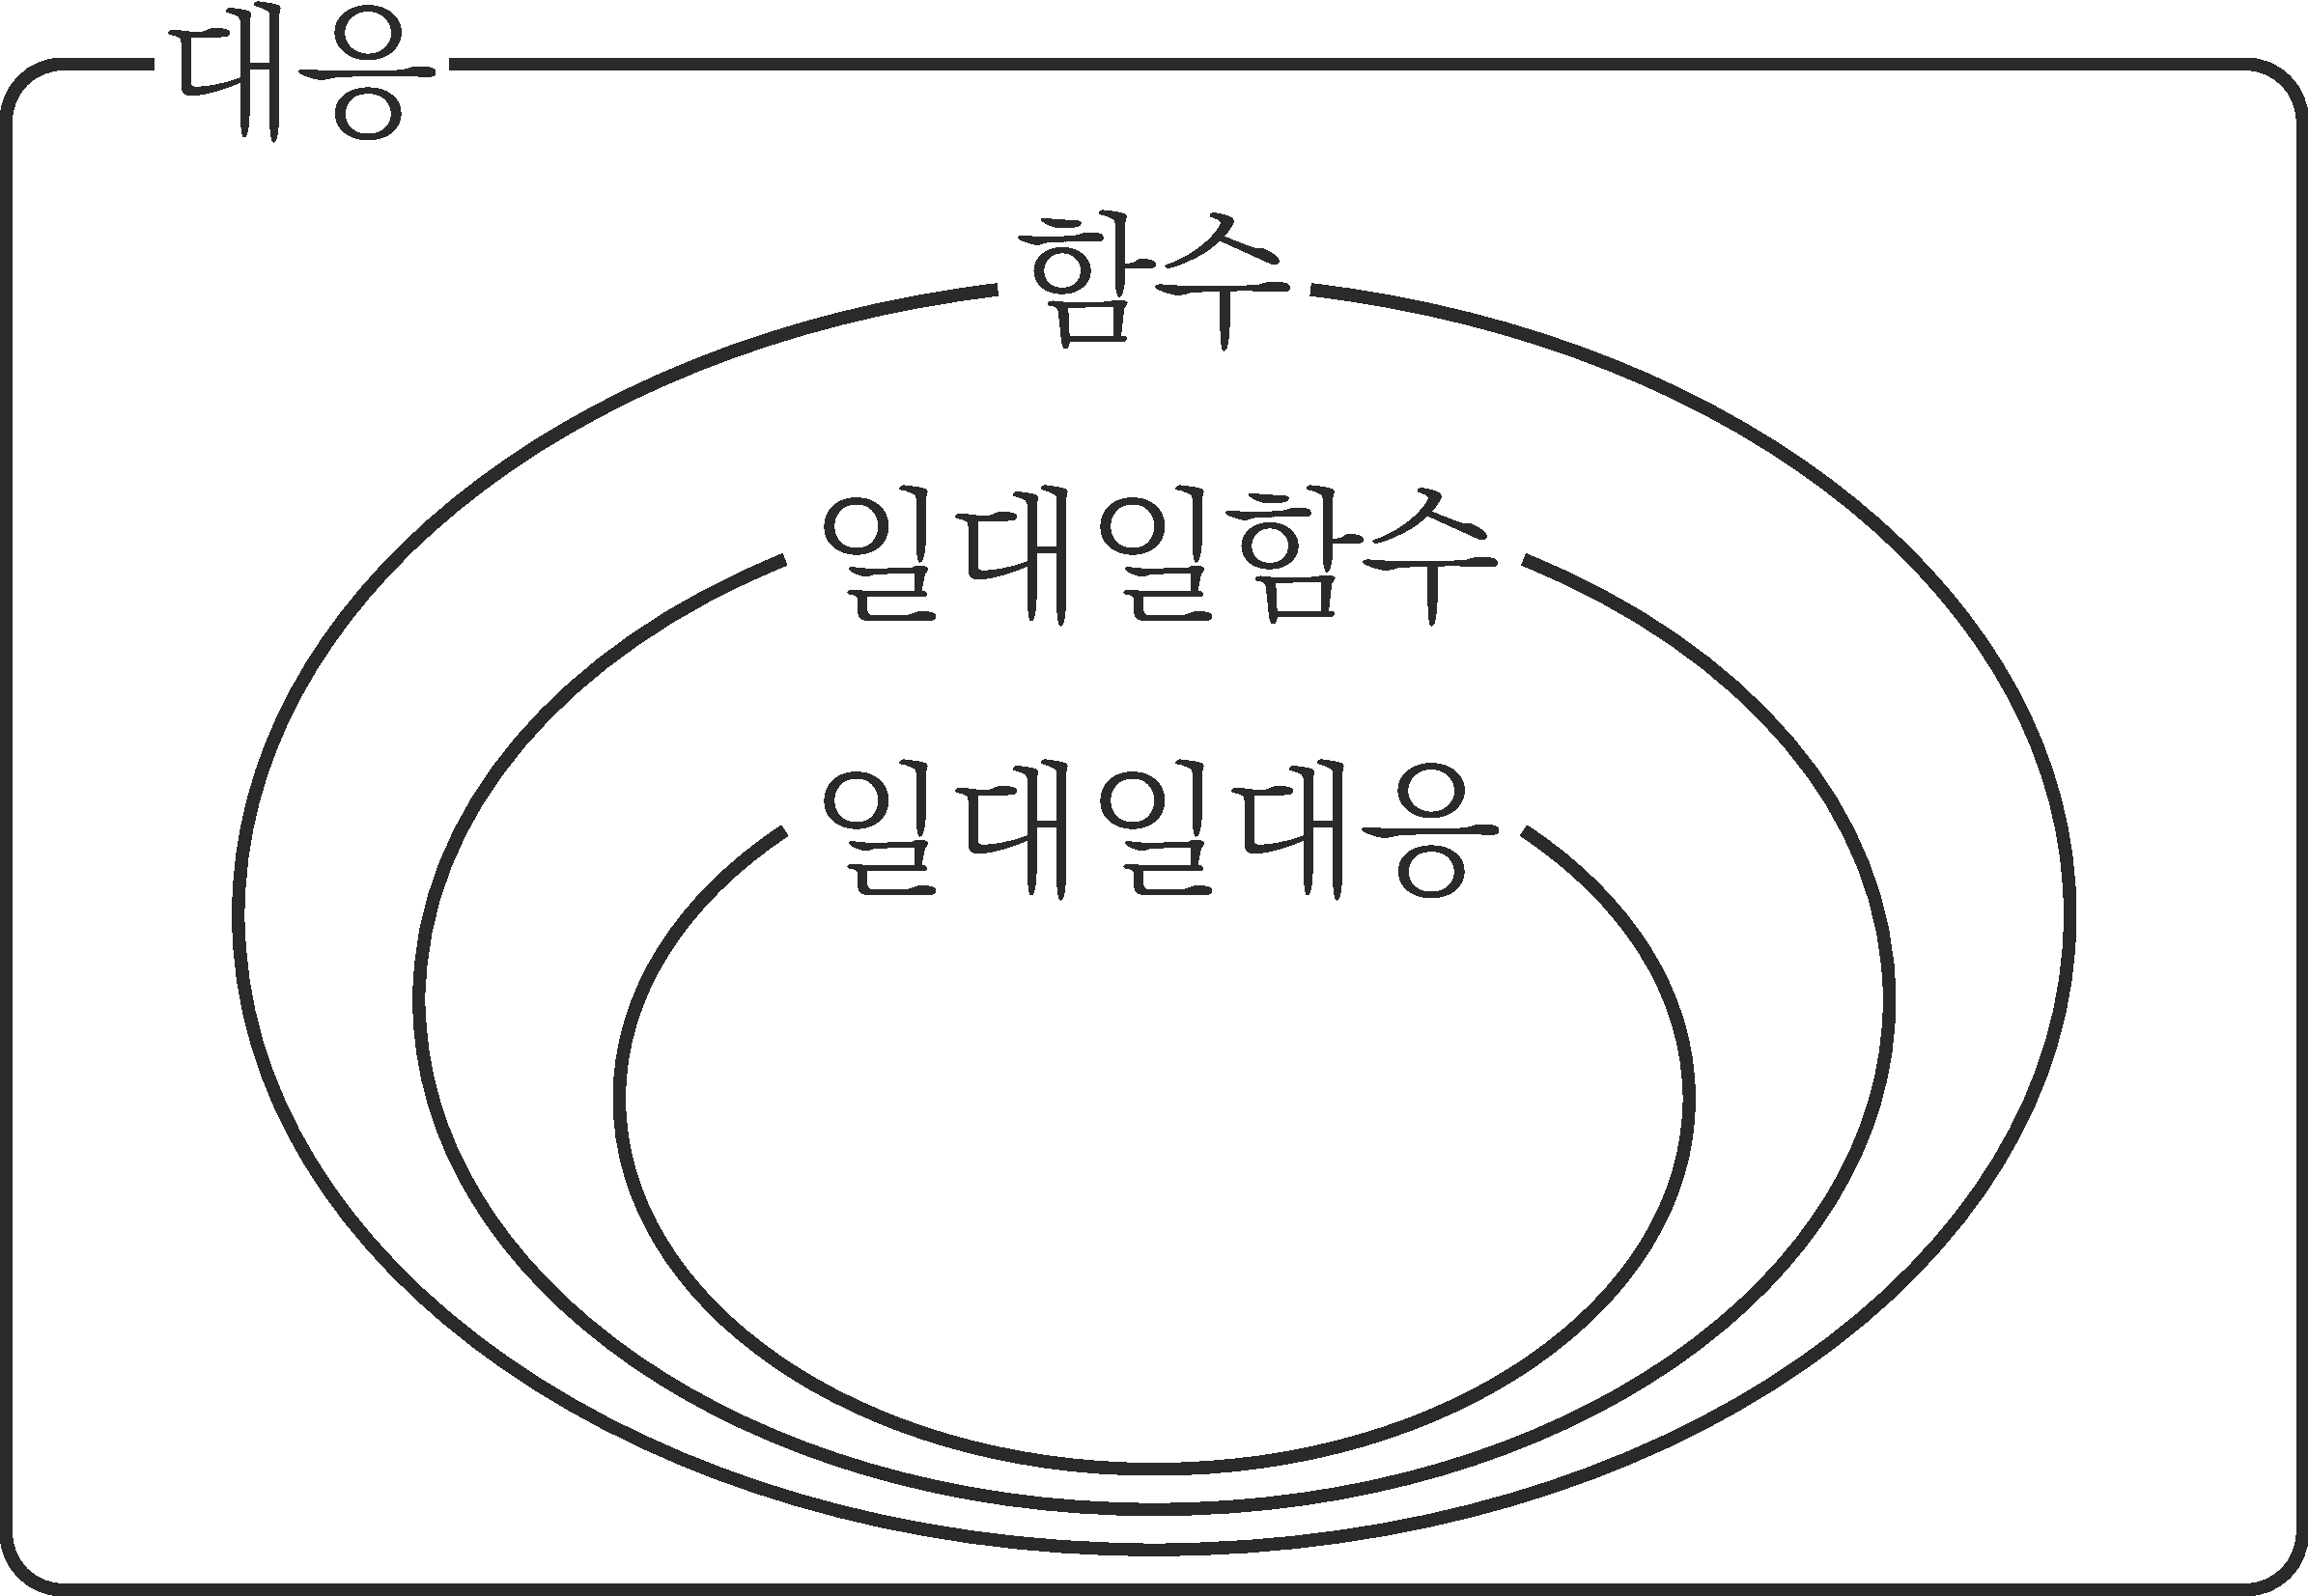
\includegraphics[scale=\pgfkeysvalueof{picsize}]{DBs/pic/zerg_02.pdf}\\
	\end{center}일대일함수, 일대일대응, 함수, 대응의 관계를 벤 다이어그램으로 나타내면 위 그림과 같습니다. 함수 $f$가 일대일대응이면 일대일함수입니다. 함수 $f$가 일대일함수이면 일대일대응일 수도 있고, 일대일대응이 아닐 수도 있습니다. 함수 $f$가 일대일함수가 아니라면 일대일대응도 아닙니다. 

\subsection{항등함수와 상수함수}
함수 $f:X \longrightarrow X$에서 정의역 $X$의 각 원소에 자기 자신이 대응할 때, 즉 $f\left( x \right) = x$일 때, 함수 $f$를 `$X$에서의 \term{항등함수}{}'라고 합니다.

함수 $f:X \longrightarrow Y$에서 정의역 $X$의 각 원소에 각각 모두 공역 $Y$의 원소 $c$가 대응할 때, 즉 $f\left( x \right) = c\:\left( \text{단, $c$는 상수} \right) $일 때, 함수 $f$를 \term{상수함수}{}라고 합니다.
\clearpage
\section{함수의 합성}
\subsection{합성함수의 정의}
일반적으로 두 함수 $f:X \longrightarrow Y$, $g:Y \longrightarrow Z$가 주어졌을 때, 집합 $X$의 임의의 원소 $x$에 대하여 함숫값 $f\left( x \right) $는 집합 $Y$의 원소이고, 집합 $Y$의 원소 $f\left( x \right) $에 대하여 함숫값 $g\left( f\left( x \right)  \right) $는 집합 $Z$의 원소입니다. 

이때 집합 $X$의 각 원소 $x$에 집합 $Z$의 원소 $g\left( f\left( x \right)  \right) $를 대응시키면, 이 대응은 $X$에서 $Z$로의 새로운 함수입니다. 이 함수를 `$f$와 $g$의 \term{합성함수}{}'라고 하며, 이것을 기호로 나타내면 다음과 같습니다.
\begin{align*} g \circ f, \quad  g \circ f : X \longrightarrow Z, \quad  y=g\left( f\left( x \right)  \right)  \end{align*}

\subsection{합성함수의 성질}
함수의 합성에서 교환법칙은 성립하지 않고, 결합법칙은 성립합니다. 따라서 여러 합성을 연달아 해야 할 때에는 아무렇게나 해서는 안 되고, 어떤 연산을 먼저 해야 결과가 최대한 간단해질 지를 따지는 것이 필요합니다.

\section{역함수}
\subsection{역함수와 원함수의 정의}
일반적으로 함수 $f:X \longrightarrow Y$가 일대일대응이면 집합 $Y$의 각 원소 $y$에 대하여 $f(x)=y$인 $X$의 원소 $x$는 단 하나 존재합니다. 이는 함수의 정의에 부합하므로, 정의역과 치역이 각각 $Y$, $X$이고\mn{교과서에서는 $X$를 공역으로 설정하고 있지만, 제약조건 (1)을 생각해보았을 때 $X$를 치역인 동시에 공역인 것으로 생각하는 것이 더 자연스러울 것입니다.}{}, $Y$의 각 원소 $y$에 $X$의 각 원소 $x$가 대응하는 새로운 함수를 생각할 수 있습니다. 이 함수를 `$f$의 \term{역함수}{}'라고 하며, 이것을 기호로 나타내면 다음과 같습니다. 
\begin{align*} f^{-1}, \quad f^{-1} : Y \longrightarrow X, \quad x=f^{-1}\left( y \right) \end{align*}

$f^{-1}$는 태생부터 함수 $f$와 매우 밀접한 관계를 가지므로, $f^{-1}$를 중심으로 생각할 때 $f$를 부를 적당한 명칭이 필요할 것입니다. 따라서 어떤 함수 $f$의 역함수 $f^{-1}$가 존재할 때, $f$를 `$f^{-1}$의 \iterm{원함수}{}'라 부르기로 합시다. 또한 $f$와 $f^{-1}$의 관계를 \iterm{역함수 관계}{}라 부르기로 합시다.

\subsection{역함수 존재성 : 일대일대응}
만약 $f:X \longrightarrow Y$가 일대일대응이 아닌 일대일함수라면, 집합 $Y$의 원소 중  $f(x)=y$인 $X$의 원소 $x$가 존재하지 않을 수 있습니다. 따라서 제약조건 (1)에 의해 함수의 정의를 만족하지 못하므로, 역함수가 존재하지 않습니다.

만약 $f:X \longrightarrow Y$가 일대일함수가 아니라면, 집합 $Y$의 원소 중 어떤 원소는 $f(x)=y$인 $X$의 원소 $x$가 여러개 존재할 수 있습니다. 따라서 제약조건 (2)에 의해 함수의 정의를 만족하지 못하므로, 역함수가 존재하지 않습니다.

\subsection{역함수와 원함수의 합성 : 서로 합성하면 항등함수}

일대일대응인 함수 $f : X \longrightarrow Y$와 $f$의 역함수 $f^{-1}$ 사이에는 다음이 성립합니다.
\begin{align*} y= f\left( x \right)  \Longleftrightarrow x=f^{-1}\left( y \right)  \end{align*}
위의 관계의 가정 명제에서, $y=f\left( x \right) $의 $x$ 대신 $x=f^{-1}\left( y \right) $를 대입하면 다음을 얻습니다.
\begin{align*} y=f\left( x \right) =f\left( f^{-1}\left( y \right) \right) = \COMP{f}{f^{-1}}{y} \end{align*}
이때 $f$는 일대일대응이므로 공역과 치역이 $Y$로 동일합니다. 따라서 $y \in Y$인 모든 원소 $y$에 대하여 $\COMP{f}{f^{-1}}{y} = y$가 성립하므로 함수 $\COMP{f}{f^{-1}}{y}$는 `$Y$에서의 항등함수'입니다. 같은 방법을 통해 함수 $\COMP{f^{-1}}{f}{x}$는 `$X$에서의 항등함수'임을 알 수 있습니다.

\subsection{새로운 함수로서의 역함수}

일반적으로 함수를 나타낼 때, 정의역의 원소를 $x$, 함숫값을 $y$로 나타내므로, 함수 $y=f(x)$의 역함수 $x=f^{-1}\left( y \right) $도 $x$와 $y$를 서로 바꾸어 $y=f^{-1}\left( x \right) $로 나타낼 필요가 있습니다. 함수 $y=f\left( x \right)$의 역함수가 존재할 때, 역함수 $y=f^{-1}\left( x \right) $는 다음과 같은 과정으로 나타낼 수 있습니다. 이러한 방법으로 얻은 새로운 함수를 \iterm{새로운 함수로서의 역함수}{}라 부르기로 합시다.
\begin{justbox}
    \begin{enumerate}[label={\onum*}]
        \item $y=f\left( x \right) $의 수식을 $x$에 관하여 나타낸다.
        \item $x$와 $y$의 위치를 서로 바꾼다.
    \end{enumerate}    
\end{justbox}

\subsection{대거역함수와 새함역함수}
역함수의 정의, 존재성, 성질에서 배웠던 `$f$의 역함수 $f^{-1}$'와, 원함수에서 $x$와 $y$를 서로 바꾸어 얻은 `새로운 함수로서의 역함수'는 이름은 역함수로 같지만 미묘한 차이가 있어 혼동의 여지가 있습니다.

이를 혼동하지 않기 위해서 전자를 `대응관계만 거꾸로인 역함수'라는 의미에서 \iterm{대거역함수}{}라 부르기로 하고, 후자를 \iterm{새함역함수}{}라 부르기로 합시다. 또한 일반적으로 역함수라 하면 새함역함수를 말하는 것으로 약속합시다. 자세한 내용은 Math I에서 다루도록 하겠습니다.
